\chapter{MVC versus Arquitetura Limpa}

    \par Este capítulo apresenta uma comparação entre a API REST original desenvolvida em MVC e sua versão refatorada com Arquitetura Limpa. A análise destaca as principais mudanças na estrutura do projeto e no fluxo das requisições, estabelecendo uma base para a compreensão dos resultados apresentados nas seções seguintes. Dessa forma, busca-se proporcionar uma visão geral da refatoração, evidenciando os impactos e aspectos que devem ser considerados na adoção da Arquitetura Limpa, os quais serão discutidos posteriormente neste trabalho.

    \par Para essa avaliação, foram definidos alguns critérios, baseados nas preocupações que motivaram a Arquitetura Limpa. Os fatores definidos para evidenciar as diferenças e semelhanças entre as abordagens são: Estrutura e Organização (que avalia o conceito de "Arquitetura Gritante" e a clareza de diretórios), Acoplamento e Coesão (medido pela aderência à Regra da Dependência e o isolamento do núcleo de negócio), Fluxo da Requisição (analisando o caminho e o número de responsabilidades por componente), e a Testabilidade/Flexibilidade (a capacidade de trocar detalhes de infraestrutura sem afetar a lógica central).
    
    \section{Comparação Estrutural}
        \par Para apresentar a materialização do modelo conceitual proposto por \cite{livro:martin:cleanarch}, a Tabela \ref{tab:mapeamento_clean_arch} apresenta o mapeamento direto entre cada componente teórico apresentado pelo autor e a sua respectiva representação no projeto, utilizando o caso de uso de criação de um novo contato como exemplo.
        
        \begin{table}[H]
            \caption{Mapeamento dos Componentes}
            \label{tab:mapeamento_clean_arch}
            \begin{tabularx}{\linewidth}{|l|X|} % Adicionados os "|" para as linhas verticais
                \toprule
                % A linha do cabeçalho foi envolvida por {\small ...} para diminuir a fonte
                {\small \textbf{Componente no Cenário Típico (Martin, 2019)}} & {\small \textbf{Classe/Artefato Implementado no Projeto}} \\
                \midrule
                Controller                  & \texttt{CreateContactController.php} \\
                Input Boundary (Interface)  & \texttt{CreateContactInputBoundary.php} \\
                Use Case Interactor         & \texttt{CreateContactInteractor.php} \\
                Input Data                  & \texttt{CreateContactRequestModel.php} \\
                Entities                    & \texttt{Contact.php} (Entidade Pura) \\
                Data Access Interface       & \texttt{ContactRepositoryInterface.php} \\
                Data Access (Implementação) & \texttt{ContactRepository.php} \\
                Database                    & MySQL (Serviço Docker) \\
                Output Boundary (Interface) & \texttt{CreateContactOutputBoundary.php} \\
                Presenter                   & \texttt{CreateContactApiPresenter.php} \\
                Output Data                 & \texttt{CreateContactResponseModel.php} \\
                View Model                  & \texttt{ContactViewModel.php} \\
                View                        & Resposta JSON \\
                \bottomrule
            \end{tabularx}
        \end{table}
       
        \par Essa tradução da teoria para a prática se inicia com o Controller, representado pela classe \texttt{CreateContactController.php}, que transforma a requisição em um Input Data, implementado como o DTO \texttt{CreateContactRequestModel.php}. Este objeto é então passado para o Use Case Interactor (\texttt{CreateContactInteractor.php}) através da Input Boundary, o contrato definido pela interface \texttt{CreateContactInputBoundary.php}. No núcleo da aplicação, o Interactor orquestra as Entities, materializadas pela classe pura \texttt{Contact.php}. 
        
        \par A persistência dos dados é abstraída pela Data Access Interface (\texttt{ContactRepositoryInterface.php}), cuja implementação concreta é o \texttt{ContactRepository.php}, que por sua vez interage com o Database (MySQL). Ao final do fluxo, o Interactor produz o Output Data (\texttt{CreateContactResponseModel.php}) e o entrega ao Presenter (\texttt{CreateContactApiPresenter.php}) através da Output Boundary (\texttt{CreateContactOutputBoundary.php}). Por fim, o Presenter formata esses dados em um View Model (\texttt{ContactViewModel.php}), que serve de base para a View, representada pela Resposta JSON final.

        \par Apresentados os componentes resultantes da aplicação da Arquitetura Limpa, pode-se realizar uma comparação entre a arquitetura MVC e a Arquitetura Limpa no contexto desse TCC, apresentando as diferenças entre a abordagem inicial, centrada no framework, e a abordagem final, centrada no domínio de negócio. 
        
        \par A primeira mudança perceptível está na organização dos diretórios. A estrutura MVC original agrupa os arquivos por seu tipo técnico (Models, Controllers), enquanto a nova estrutura os organiza por camadas e funcionalidades, refletindo o conceito de "Arquitetura Gritante".
        
        \par Nesse sentido, nota-se que a API base, seguindo o padrão Laravel, possuía uma estrutura enxuta, com a lógica de negócio, acesso a dados e controle de requisições concentradas principalmente nos diretórios \texttt{app/Http/Controllers} e \texttt{app/Models}, conforme consta na Figura~\ref{fig:estrutura-original} onde é apresentada a estrutura do diretório \texttt{app} da API REST base. 

        \begin{figure}[H]
            \caption{Estrutura do diretório app antes da refatoração.}
            \label{fig:estrutura-original}
            \dirtree{%
            .1 app/.
            .2 Http/.
            .3 Controllers/.
            .4 ContactController.php.
            .4 Controller.php.
            .2 Models/.
            .3 Contact.php.
            .3 User.php.
            .2 Providers.
            .3 AppServiceProvider.php.
            }
        \end{figure}

        \par Já após a refatoração, a estrutura de diretórios passou a refletir as camadas da Arquitetura Limpa. As regras de negócio agora residem em \texttt{app/Entities} e \texttt{app/UseCases}, completamente isoladas do framework. Os componentes que interagem com o mundo externo, como Controllers e Repositories, foram movidos para \texttt{app/InterfaceAdapters}, e os detalhes de implementação específicos do Laravel, como os Models do Eloquent, para \texttt{app/FrameworksAndDrivers}. A Figura \ref{fig:estrutura-depois} demonstra a organização final do diretório \texttt{app}.

        \begin{figure}[H]
            \caption{Estrutura do diretório app após a refatoração.}
            \label{fig:estrutura-depois}
            \dirtree{%
            .1 /app.
            .2 Entities.
            .3 Contact.php.
            .2 FrameworksAndDrivers.
            .3 Models.
            .4 ContactModel.php.
            .3 Providers.
            .4 AppServiceProvider.php.
            .4 CleanArchServiceProvider.php.
            .2 InterfaceAdapters.
            .3 Http.
            .4 Controllers.
            .5 Controller.php.
            .5 Contact.
            .6 CreateContactController.php.
            .6 ....
            .3 Presenters.
            .4 Api.
            .5 CreateContactApiPresenter.php.
            .5 ....
            .3 Repositories.
            .4 ContactRepository.php.
            .3 ViewModels.
            .4 ContactViewModel.php.
            .2 UseCases.
            .3 Contracts.
            .4 ContactRepositoryInterface.php.
            .3 CreateContact.
            .4 CreateContactInteractor.php.
            .4 Boundaries.
            .5 CreateContactInputBoundary.php.
            .5 CreateContactOutputBoundary.php.
            .4 DTOs.
            .5 CreateContactRequestModel.php.
            .5 CreateContactResponseModel.php.
            .3 Exceptions.
            .4 BusinessRuleException.php.
            .4 ResourceNotFoundException.php.
            .3 ....
        }
        \end{figure}

        \par Essa nova organização deixa explícito o propósito da aplicação (gerenciar contatos, com casos de uso como CreateContact, etc.) antes mesmo de revelar qual tecnologia é usada para isso.

    \section{Comparação do fluxo da Requisição}

    \par O fluxo da Arquitetura MVC Original, ilustrado na Figura~\ref{fig:mvc1}, é direto e revela um alto nível de acoplamento ao \textit{framework}, violando o Princípio da Responsabilidade Única. A requisição HTTP (\texttt{POST /contacts}) é recebida pela Rota, que a encaminha ao \texttt{ContactController}. O \textit{Controller} é então ativado e assume múltiplas responsabilidades simultaneamente: ele instancia diretamente o \texttt{ContactModel} (Eloquent), criando um forte acoplamento ao ORM, e define seus atributos com os dados brutos da requisição HTTP. 
    
    \par Em seguida, o \textit{Controller} chama o método \texttt{save()} do \textit{Model}, orquestrando a persistência de dados no Banco de Dados. Esse comportamento fez com que o \textit{Controller} atue como manipulador de HTTP, orquestrador de lógica de negócio e componente de acesso a dados. O fluxo é finalizado com o \textit{Controller} retornando a resposta JSON ao Cliente, acumulando também a responsabilidade de formatação da saída (\textit{Presenter}).

    \par Com a refatoração, o fluxo (Figura~\ref{fig:ca1}) inverte as dependências, garantindo que o núcleo da aplicação seja totalmente isolado. O processo começa com o \texttt{Controller} (Adaptador de Interface) recebendo a requisição HTTP (1). Seu papel é estritamente limitado à tradução da entrada: ele cria o \texttt{RequestModel} (DTO) (2) e invoca o Caso de Uso através da interface \texttt{InputBoundary} (3), passando o DTO agnóstico e uma instância do \texttt{Presenter}.

    \par O \texttt{Interactor} (Caso de Uso) é ativado na camada de lógica de negócio. Sua responsabilidade é puramente a execução da regra: ele cria e valida a \texttt{Entidade Contact} (4) e, para persistir, chama a \texttt{ContactRepositoryInterface} (5). A Regra da Dependência é estritamente obedecida, pois o \textit{Interactor} não conhece o \textit{framework} ou o ORM. A implementação concreta do repositório interage com o Banco de Dados (6, 7, 8) e retorna a \texttt{Entidade Salva} para o \textit{Interactor}.

    \par O \texttt{Interactor} cria o \texttt{ResponseModel} (DTO de saída) (9) e o envia ao \texttt{Presenter} através da \texttt{OutputBoundary} (10), finalizando a lógica de negócio. O \texttt{Presenter} (Adaptador de Saída) formata os dados brutos no \texttt{ViewModel} (11). O \texttt{Controller} (Adaptador de Entrada) recupera o \texttt{ViewModel} (13, 14) e envia a resposta JSON (15). Essa segregação de tarefas, ao isolar a lógica de negócio na camada de \textit{Use Cases}, torna o núcleo da aplicação totalmente testável em unidade (sem dependência do \textit{framework}, \textit{HTTP} ou Banco de Dados) e flexível a alterações de tecnologia externa.

    \begin{figure}[H]
        \centering
    
        \begin{minipage}{0.49\linewidth}
            \centering
            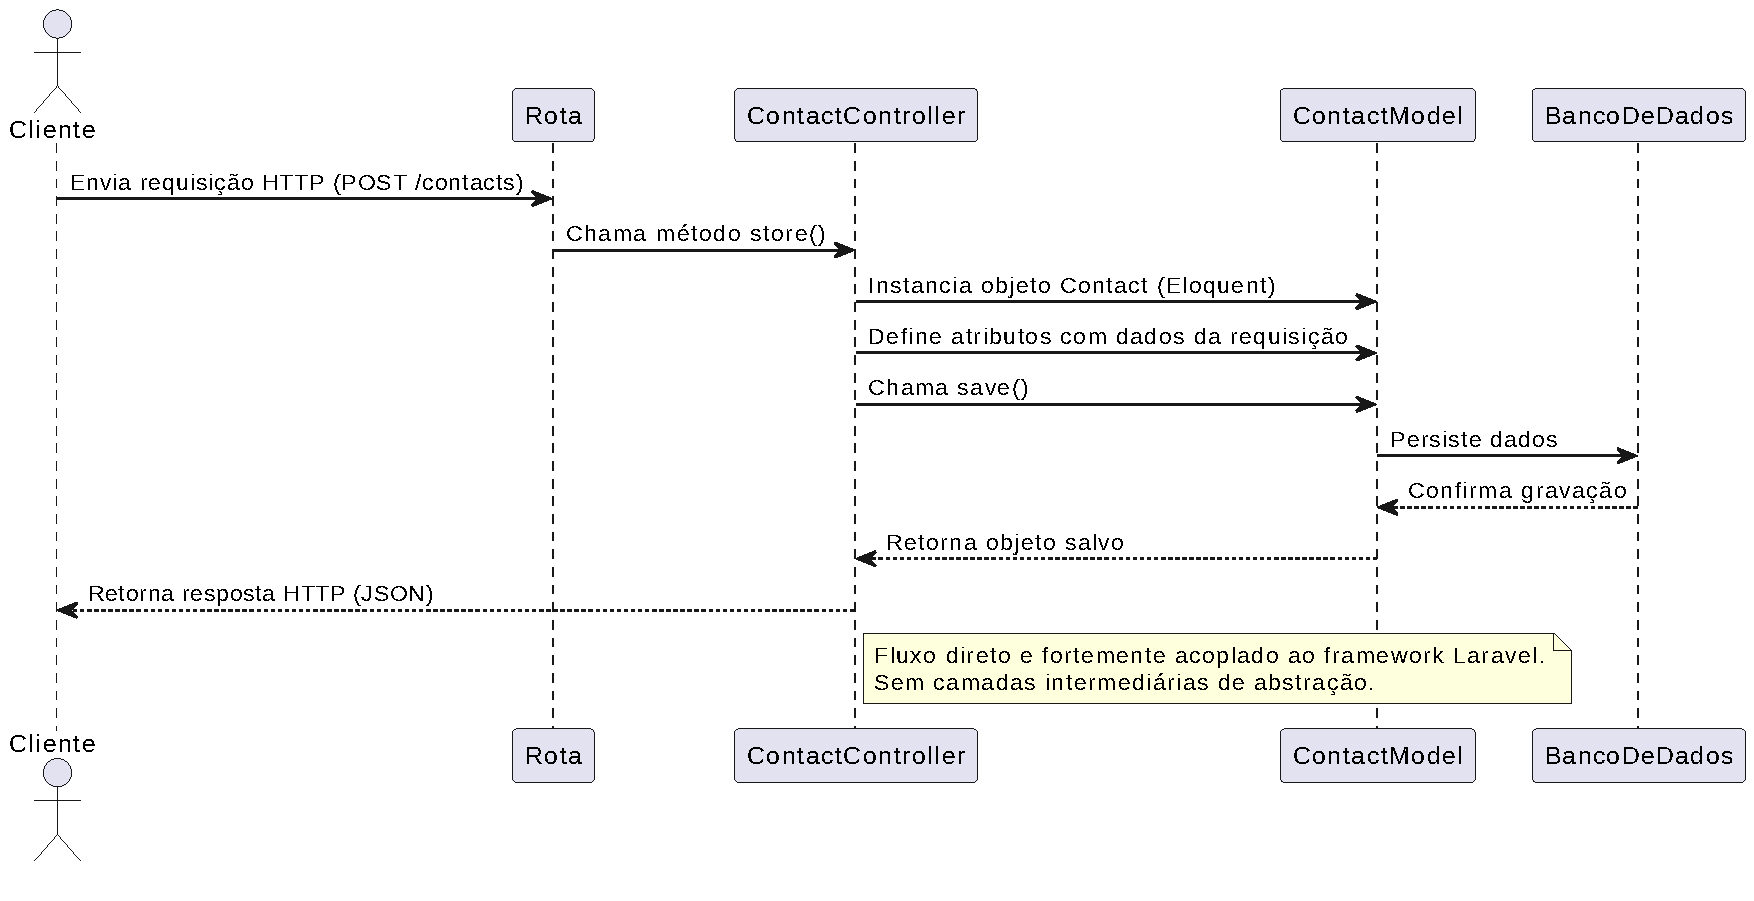
\includegraphics[angle=-90,width=1.0\linewidth]{figuras/resultados/mvc1.pdf}
            \caption{Fluxo da Requisição - Arquitetura MVC Original (Laravel).}
            \label{fig:mvc1}
            
        \end{minipage}
        \hfill
        \begin{minipage}{0.49\linewidth}
            \centering
            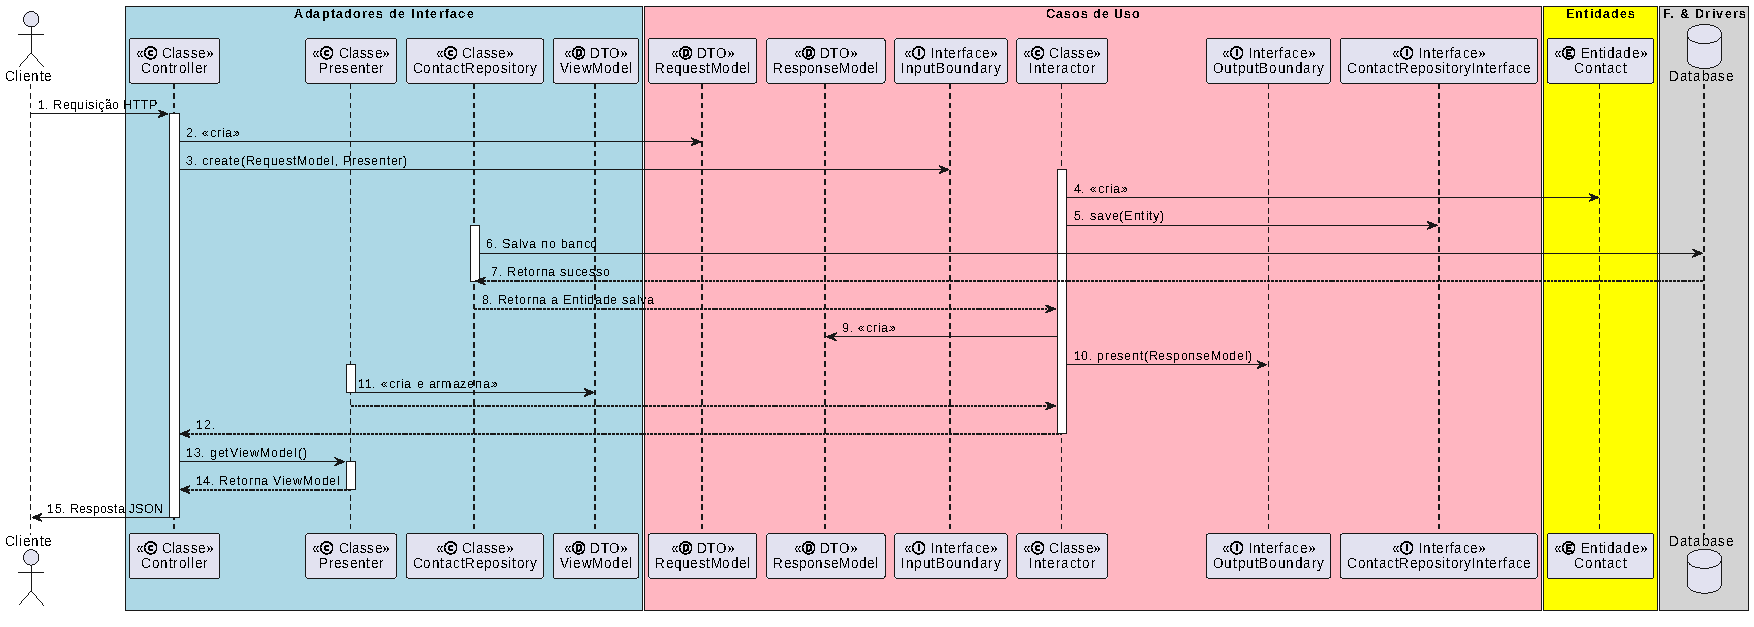
\includegraphics[angle=-90,width=1.0\linewidth]{figuras/resultados/ca1.pdf}
            \caption{Fluxo da Requisição - Arquitetura Limpa (Laravel).}
            \label{fig:ca1}
            
        \end{minipage}
    \end{figure}

    \vspace{1cm}


    \par Diante dessa comparação, pode-se notar que o padrão MVC não foi descartado, mas sim reposicionado. No modelo original da API REST no Laravel, o Controller e o Model atuavam de forma acoplada, concentrando tanto a adaptação da requisição HTTP, quanto a lógica de negócio e a persistência de dados.

    \par Diferentemente, com a Arquitetura Limpa, essa concentração de responsabilidades foi desmembrada e realocada, alinhando-se aos princípios SOLID e à Regra da Dependência. O Controller foi movido para a camada de Adaptadores de Interface, assumindo a única função de traduzir a requisição HTTP em um RequestModel (DTO) e invocar o Caso de Uso correspondente.

    \par Já o Model foi isolado na camada mais externa de Frameworks e Drivers, enquanto sua lógica essencial de domínio foi migrada para a classe pura da Entidade (Contact.php) e para o Interactor, que representa o novo núcleo de negócio (Caso de Uso).

    \par O resultado é que o padrão MVC passou a operar estritamente como a camada de interação externa, adaptando as entradas e saídas (com o auxílio do Presenter e ViewModel para a View JSON), enquanto o núcleo de negócio permanece completamente isolado e agnóstico ao framework.